\chapter{Introducción}
\label{cap:capitulo1}
\setcounter{page}{1}

El ictus es una enfermedad cerebro-vascular (ECV).
El término ictus en latín significa golpe.
Es un trastorno brusco de la circulación cerebral que altera la función de una determinada región del cerebro.\\

Según la Organización Mundial \cite{cita1} (OMS) es la primera causa de discapacidad y la segunda de muerte en el mundo.
Aproximadamente 15 millones de personas sufren un ictus cada año; entre ellas, 5 millones mueren y otros 5 millones quedan con alguna discapacidad permanente, lo que supone una carga significativa para las familias y comunidades, como indica la \cite{cita2}.\\

Las causas o factores de riesgo según la Federación Española \cite{cita3} son las siguientes:
\begin{enumerate}
    \item Sufrir un ictus recientemente.
	\item Presión sanguínea elevada.
	\item Fumar.
	\item Padecer diabetes.
	\item Sufrir una enfermedad cardiaca.
	\item Estación del año y clima.
	\item Contador de glóbulos rojos alto.
	\item Consumo excesivo de alcohol y drogas.\\
\end{enumerate}\

Según el Sistema Nacional de Salud, \cite{perales1a}, cada año, alrededor de $120.000$ personas sufren un ictus en España.
La edad es uno de los factores de riesgo principales de esta enfermedad, aunque ocurre en todos los grupos de edad.
En los últimos años la incidencia en adultos jóvenes ha aumentado un $40\%$.
Se estima que 1 de cada 4 personas en el mundo sufrirán un ictus a lo largo de su vida.
Gracias a los avances científicos, tecnológicos y clínicos se han podido desarrollar tratamientos para minimizar los déficit que produce.
En la Imagen \ref{fig:grafica}, se muestra la prevalencia registrada de enfermedad cerebro-vascular por 1.000 habitantes, según sexo y edad en España en 2019.
Y, en la Imagen \ref{fig:grafica2}, se pueden observar datos sobre la incidencia del ictus en España en el año 2020.\\

\begin{figure}[ht!]
	\centering
	\begin{minipage}{0.65\linewidth}
		\centering
		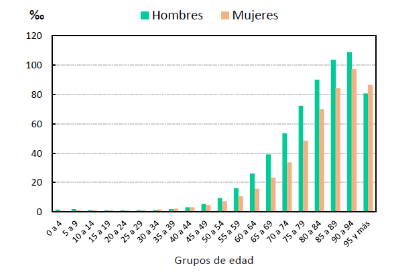
\includegraphics[width=\linewidth]{figs/edad_ictus_es.png}
	\end{minipage}
	\caption[Prevalencia registrada de enfermedad cerebro-vascular según sexo y edad en España, 2019]{Fuente: Figura extraída del Informe Anual de Salud del Sistema Nacional de Salud 2020-2021.
	Fuente de datos: Ministerio de Sanidad. Base de Datos Clínicos de Atención Primaria (BDCAP)}
	\label{fig:grafica}
\end{figure}

\begin{figure}[ht!]
	\centering
	\begin{minipage}{0.65\linewidth}
		\centering
		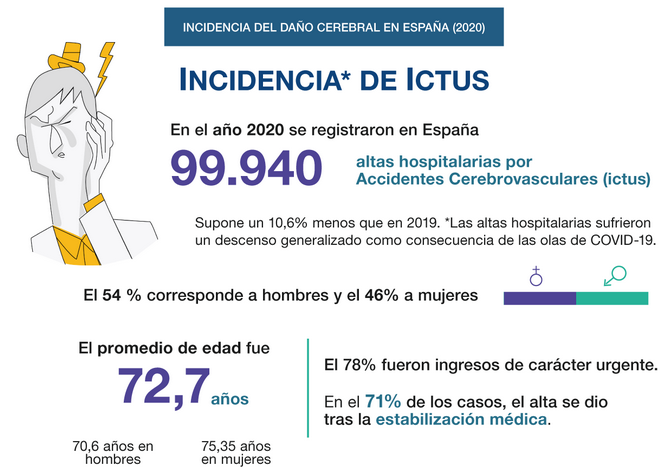
\includegraphics[width=\linewidth]{figs/incidencia_ictus_es.png}
	\end{minipage}
	\caption[Incidencia del ictus en España, 2020]{Fuente de datos: Encuesta de Movilidad Hospitalaria (INE, 2020). Ministerio de España. FEDACE. Observatorio Estatal Daño Cerebral}
	\label{fig:grafica2}
\end{figure}

\vspace{1cm}
Según la OMS, la rehabilitación se define como un $"$conjunto de medidas que ayudan a las personas que tienen o probablemente tendrán una discapacidad, a conseguir y mantener el funcionamiento óptimo en interacción con su ambiente".\\

Asimismo el Grupo de Estudio de ECV de la Sociedad Española de Neurología, \cite{perales1}, considera que la rehabilitación es una de las partes más importantes para el tratamiento de la mayoría de los pacientes que han sufrido un ictus y han sobrevivido.
Suele comenzarse en los primeros días de estancia en el hospital y se recomienda a cualquier paciente que, previo al ictus, fuese autosuficiente.
Es importante entender que es difícil volver a una situación igual a la inicial.
El objetivo fundamental es ayudar al paciente a adaptarse, ya que el ictus se recupera de forma espontánea o puede no recuperarse nunca, dependiendo de su gravedad, la cual determina la duración del programa de rehabilitación y su intensidad.
Los seis primeros meses son los de mayor importancia para recuperar los movimientos voluntarios.
Con un programa adecuado, $1/3$ de los pacientes vuelven a su trabajo.\\

El plan de acción europeo para el ictus 2018-2030, propuesto por la Alianza Europea contra el ictus \cite{perales2a}, surge con el objetivo de mejorar el cuidado de los ictus y la vida después de estos.
Entre los objetivos generales para el año 2030 se encuentran:
\begin{enumerate}
    \item Garantizar que al menos el $90\%$ de la población tenga acceso a la rehabilitación precoz en la unidad de ictus.
    \item Proporcionar el alta precoz con apoyo a por lo menos el $20\%$ de los pacientes de ictus en todos los países.
    \item Ofrecer programas de acondicionamiento físico a todos los pacientes de ictus que viven en la comunidad.
    \item Proporcionar un plan documentado para la rehabilitación en la comunidad y el apoyo al autocontrol de todos los pacientes de ictus con dificultades residuales al recibir el alta hospitalaria.
    \item Garanticen que se revisan las necesidades de rehabilitación, y otras, de todos los pacientes de ictus entre los 3 y 6 meses después de sufrirlo y anualmente a partir de ese momento.\\
\end{enumerate}\

La Sociedad Española \cite{cita5} (SERMEF), redacta que el $50\%$ de los supervivientes de ictus sufre secuelas y la rehabilitación temprana reducirá su dependencia en un $20\%$.
Además, manifiesta que existen desigualdades en los accesos a estos tratamientos entre Comunidades Autónomas.
Entre las principales secuelas se encuentra la pérdida de función motora, que afecta entre el $50\%$ y $85\%$ de los pacientes, trastornos del habla, disfunciones cognitivas, eplasticidad y debilidad muscular.\\

Una vez conocida la prevalencia del ictus y la importancia de la rehabilitación, se valoran las ventajas de introducir la robótica en este campo.

En el artículo de \cite{perales3a}, se analizaban los beneficios de la rehabilitación asistida por robots frente a la fisioterapia tradicional.
Esta consiste en la realización de ejercicios manuales por parte de un fisioterapeuta cualificado, aunque son muy exigentes en cuanto al tiempo de dedicación al paciente.
El uso de terapias mediadas por robots podría mejorar sustancialmente la recuperación de la función tras un ictus y, a su vez, reducir las exigencias impuestas a terapeutas y hospitales.
Por ello se comenzó una investigación para utilizar dispositivos mecánicos en el proceso de rehabilitación.\\

Varios autores han propuesto el uso de dispositivos robóticos para la rehabilitación del miembro superior.
Existen diversos modelos como el robot MIT-MANUS o Gentle/s.

El primero, fue desarrollado por los investigadores \cite{perales3b}, Volpe y Hogan, del Massachusetts Institute of Technology y del Burke Medical Research Institute.
Se ha demostrado que reduce de manera eficaz el tiempo de recuperación motriz del paciente al realizar los ejercicios apropiados para la rehabilitación del hombro y el codo.
En la Imagen \ref{fig:mitmanus}, se puede observar un paciente hospitalizado por ictus durante la terapia en el Hospital de Rehabilitación Burke (White Plains, NY), llevada a cabo con una versión comercial de MIT-MANUS.

\begin{figure}[ht!]
	\centering
	\begin{minipage}{0.55\linewidth}
		\centering
		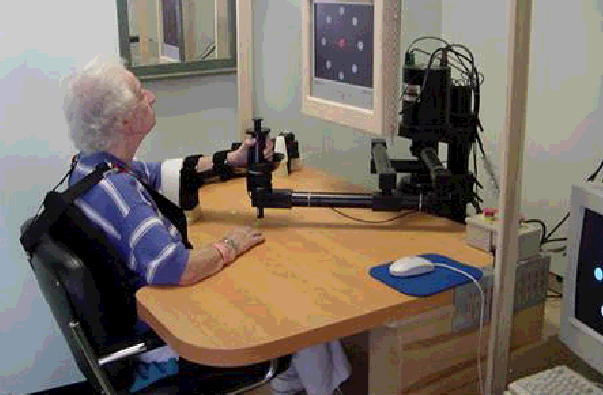
\includegraphics[width=\linewidth]{figs/mit_manus.png}
	\end{minipage}
	\caption[Terapia asistida por el robot MIT-MANUS]{Fuente: Robótica de rehabilitación: prueba piloto de una extensión espacial para MIT-Manus}
	\label{fig:mitmanus}
\end{figure}

El segundo, es un robot de asistencia robótica en rehabilitación neurológica y motora.
Como se indica en el artículo \cite{perales3c}, la tasa de recuperación fue mayor durante la fase de terapia mediada por el robot que en la fase base para la mayoría de los sujetos.
En la Imagen \ref{fig:gentles}, se muestra a un usuario utilizando el prototipo comercial Gentle/s.\\

\begin{figure}[ht!]
	\centering
	\begin{minipage}{0.55\linewidth}
		\centering
		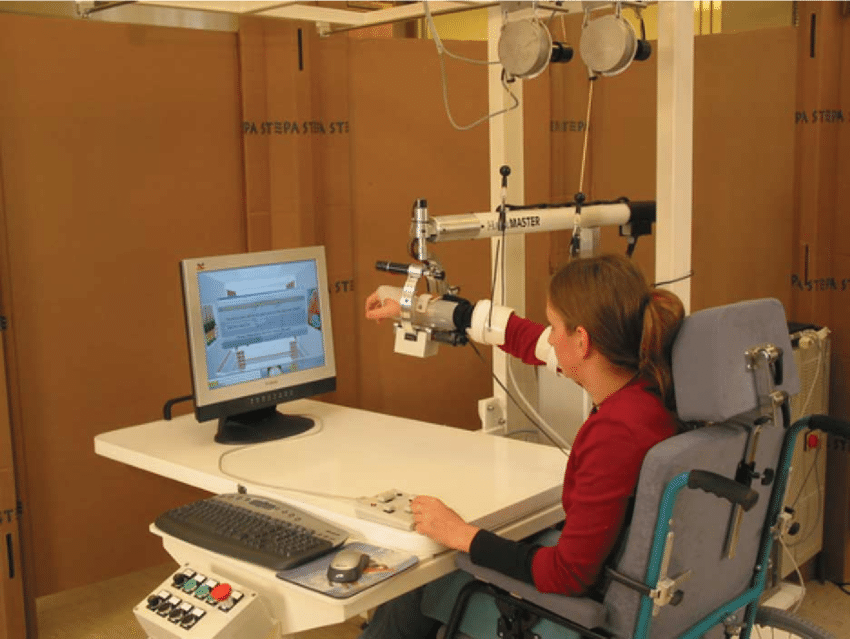
\includegraphics[width=\linewidth]{figs/gentles.png}
	\end{minipage}
	\caption[Prototipo comercial del robot rehabilitador Gentle/s]{Fuente: Retos y oportunidades de la neurorrehabilitación asistida por robots. ResearchGate}
	\label{fig:gentles}
\end{figure}

Según \cite{perales3d}, la rehabilitación asistida por robot ofrece ventajas importantes respecto a la fuerza muscular, el aumento de las puntuaciones clínicas y un grado mayor de recuperación de la independencia funcional.\\

En los últimos $5$ años, se han realizado distintos análisis sobre la efectividad de la incorporación robótica en la rehabilitación.

\begin{itemize}
	\item En el artículo \cite{perales4a} se realiza un metanálisis para medir el rendimiento de las extremidades superiores de $18$ estudios. Concluyó que la rehabilitación con brazo robótico y una duración de entre $30$ y $60$ minutos por sesión, mejoraron significativamente la función de las extremidades superiores.
	\item En el artículo \cite{perales4b} se indica que la terapia con robots es una terapia relativamente nueva, permite aumentar el número de repeticiones en la ejecución de movimientos específicos y concluyen que presenta beneficios en todas las fases de rehabilitación del ictus.
	\item En el artículo \cite{perales4c} se realiza una búsqueda para analizar el efecto de los robots de rehabilitación seleccionando $18$ ensayos con $573$ pacientes con ictus y los resultados mostraron que los pacientes que reciben este tipo de terapia mejoraron significativamente las puntaciones de evaluación motora. Concluyeron que el entrenamiento asistido por robot es superior al entrenamiento convencional, lo que respalda el uso de robots en la práctica clínica.
\end{itemize}\

Las técnicas de gamificación no son solamente lúdicas, sino que deben conseguir mejorar el aprendizaje.
Para ello, se incluyen diversos elementos como son: el objetivo del juego, distintos tipos de obstáculos y retos para incentivar un mayor esfuerzo por parte del paciente, promoviendo su superación, y recompensas para generar un refuerzo positivo en su progreso y fomentar su motivación.
La gamificación mejora la salud de los pacientes mejorando los ámbitos de vida, fomentando el cumplimiento del tratamiento, facilitando el diagnóstico de la enfermedad, mejorando la salud psicológica y ralentizando el deterioro cognitivo, como se explica en \cite{cita6}.\\

Para que la rehabilitación del paciente no resulte monótona y desmotivadora, es interesante incluir entornos gamificados en las terapias como refleja \cite{perales5a}.
Con ello se consigue un mejor compromiso y adherencia, un incremento de la motivación del paciente y permite la personalización del ejercicio.\\

Como explica \cite{perales5b} los dispositivos gamificados se pueden clasificar en cuatro tipos: robótica monitorizada, no monitorizada, realidad virtual y estimulación eléctrica neuromuscular.
La conclusión del estudio recoge que los pacientes tuvieron un impacto positivo significativo en los niveles emocional, social y personal, además de una mejora en su función motora y cognitiva.\\

Aplicado a la práctica, se realizó un estudio por \cite{perales5c} que consistió en la rehabilitación del brazo gamificada para personas con ictus.
El juego se personaliza según la capacidad de cada paciente y aumenta su dificultad en función del rendimiento del individuo.
El objetivo del estudio fue evaluar si $10$ días de entrenamiento gamificado mejora la velocidad de la recuperación motora del brazo.
Los datos del estudio sugieren que las intervenciones de rehabilitación motora gamificadas pueden beneficiar el comportamiento motor después de un accidente cerebro-vascular.\\

Algunos juegos y plataformas utilizadas en la actualidad para rehabilitación motora post-ictus son los siguientes:
\begin{itemize}
	\item Sistema de Estimulación para Promover la Independencia mediante Kinect (EPIK), desarrollado por investigadores del Grupo de Telemática e Imagen (GTI) de la Universidad de Valladolid (UVa). Basado en el sensor Kinect con el objetivo de realizar ejercicios de equilibrio. La noticia fue publicada por \cite{cita7}. En la Imagen \ref{fig:epik} se muestra el funcionamiento del sistema de rehabilitación EPIK como un videojuego 3D basado en la imitación de siluetas.

	\begin{figure}[ht!]
		\centering
		\begin{minipage}{0.55\linewidth}
			\centering
			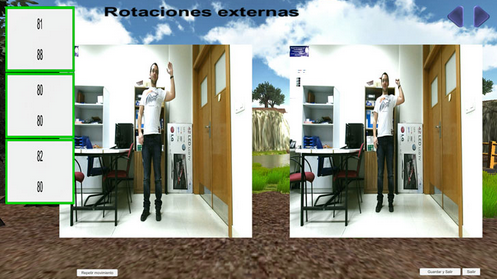
\includegraphics[width=\linewidth]{figs/EPIK.png}
		\end{minipage}
		\caption[Sistema de rehabilitación EPIK]{Fuente: \cite{cita7}}
		\label{fig:epik}
	\end{figure}

	\item Peter Jumper y Andrómeda son dos videojuegos desarrollados por la Universidad Carlos III en colaboración con a Escuela Politécnica del Ecuador y los hospitales ASEPEYO en Barcelona y Madrid. Se trata de un sistema de rehabilitación para personas con problemas de movilidad en mano y muñeca. Permite analizar la evolución del paciente mediante los datos biométricos generados. Publicado por \cite{cita8}. En la Imagen \ref{fig:videogamesuc3m} se observa a un usuario con el controlador manejando el videojuego \textit{Peter Jumper}.\\

	\begin{figure}[ht!]
		\centering
		\begin{minipage}{0.55\linewidth}
			\centering
			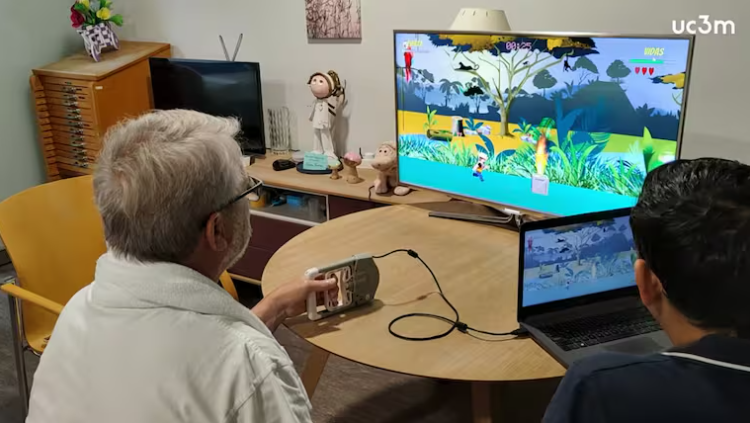
\includegraphics[width=\linewidth]{figs/uc3m_game.png}
		\end{minipage}
		\caption[Videojuego Peter Jumper para la rehabilitación de manos y muñecas]{Fuente: \cite{cita8}}
		\label{fig:videogamesuc3m}
	\end{figure}

	\item Proyecto Multi-sensorial Immersive Dynamic Autonomous System (MIDAS), compuesto por un exoesqueleto de mano, un subsistema de realidad virtual (RV) y un subsistema olfativo. En su conjunto involucra cuatro de los cinco sentidos durante la rehabilitación. Puede encontrarse publicado en \cite{cita9}.
\end{itemize}\

Una vez realizada una revisión sobre el ictus, los métodos de rehabilitación, la gamificación y la importancia de su aplicación en la recuperación del paciente, se plantea la necesidad de crear un proyecto para la rehabilitación motora de la extremidad superior mediante una plataforma robótica gamificada.
Este proyecto se enfoca en el diseño de la arquitectura software, compuesta por interfaces gráficas para el control y configuración de los parámetros terapéuticos y visualización del rendimiento del paciente.
Asimismo, se desarrolla un videojuego para fomentar la motivación y atención del paciente, que puede personalizar el terapeuta según las necesidades de cada usuario.
